\documentclass{article}
\usepackage[utf8]{inputenc}
\usepackage{graphicx}
\usepackage{url}
\graphicspath{ {./images/} }

\title{Constructing a Connectome for Alzheimer's Treatment}
\author{Ajay Ananthakrishnan, Elizabeth Daramola, Kevin Drucia, Carolyn Marar }
\date{January 2020}

\begin{document}

\maketitle

\section{Scientific Question}
Alzheimer's disease (AD) is an untreatable neurodegenerative disorder which impairs a person's ability to think, recall memories, and perform basic tasks. Around 5.5 million Americans are estimated to suffer from AD, suggesting that this disease may be the third leading cause of death in the elderly. \cite{Alzheimer's Facts} While treatments are being developed for other neurodegenerative diseases with limited success, there are currently no treatments for AD. As the population ages, AD is becoming an urgent public health issue in need of a solution.

Deep Brain Stimulation (DBS) is a therapeutic technique in which electrodes are implanted into the brain. Electrical signals are used to stimulate the surrounding neurons and regulate abnormal behavior. DBS has been approved for a number of ailments \cite{DBS uses}, and it has been shown to significantly improve symptoms of Parkinson's disease. \cite{DBS PD} Little research has been done on the effects of DBS in AD. One study saw no significant improvement in cognitive tests of AD patients after DBS of the fornix. \cite{DBS AD} Much more research must be conducted before ruling DBS therapy out for AD treatment, though. DBS may prove more effective in a different region of the brain. Our study aims to determine if this is the case.

This study aims to create a predictive algorithm that models the progression of Alzheimer’s disease and connectivity throughout disease progression. This model will then be used to pinpoint optimal points of stimulation for DBS treatment in patients. Specifically, we aim to create a model that simulates the creation and spread of amyloid beta and tau pathology throughout the brain in AD progression. We hope to do this by combining out generated MRI and DTI data with the expression of certain proteins associated with Alzheimer’s such as PS1 to create a novel predictive model of AD disease. Then, certain nodes (or brain regions) will be stimulated and it will be determined which nodes are optimal points of stimulation by comparing the predictive connectome before and after stimulation). This will help us understand optimal points of stimulation via DBS in actual Alzheimer’s patients.

\section{Hardware and Facilities}
For the purposes of this experiment, we will utilize an MRI machine for imaging humans as well as an MRI machine of a stronger imaging capacity for imaging mice. The total of these two machines will total approximately 1,500,000 dollars. Additionally, the maintenance of these MRI machines will be approximately 20,000 dollars per year. We plan to buy 100 mice, and split them into four cohorts. The cost of these mice will total approximately 10,000 dollars. Next, the cost of one DBS electrode is approximately 6000 dollars. As we plan to implant 52 human patients with electrodes, and approximately 80 mice, the total cost of 132 electrodes will be approximately 800,000. Lastly, we will need an operating and postoperative recovery room in which human patients can recover. 

\begin{figure}[!]
\centering
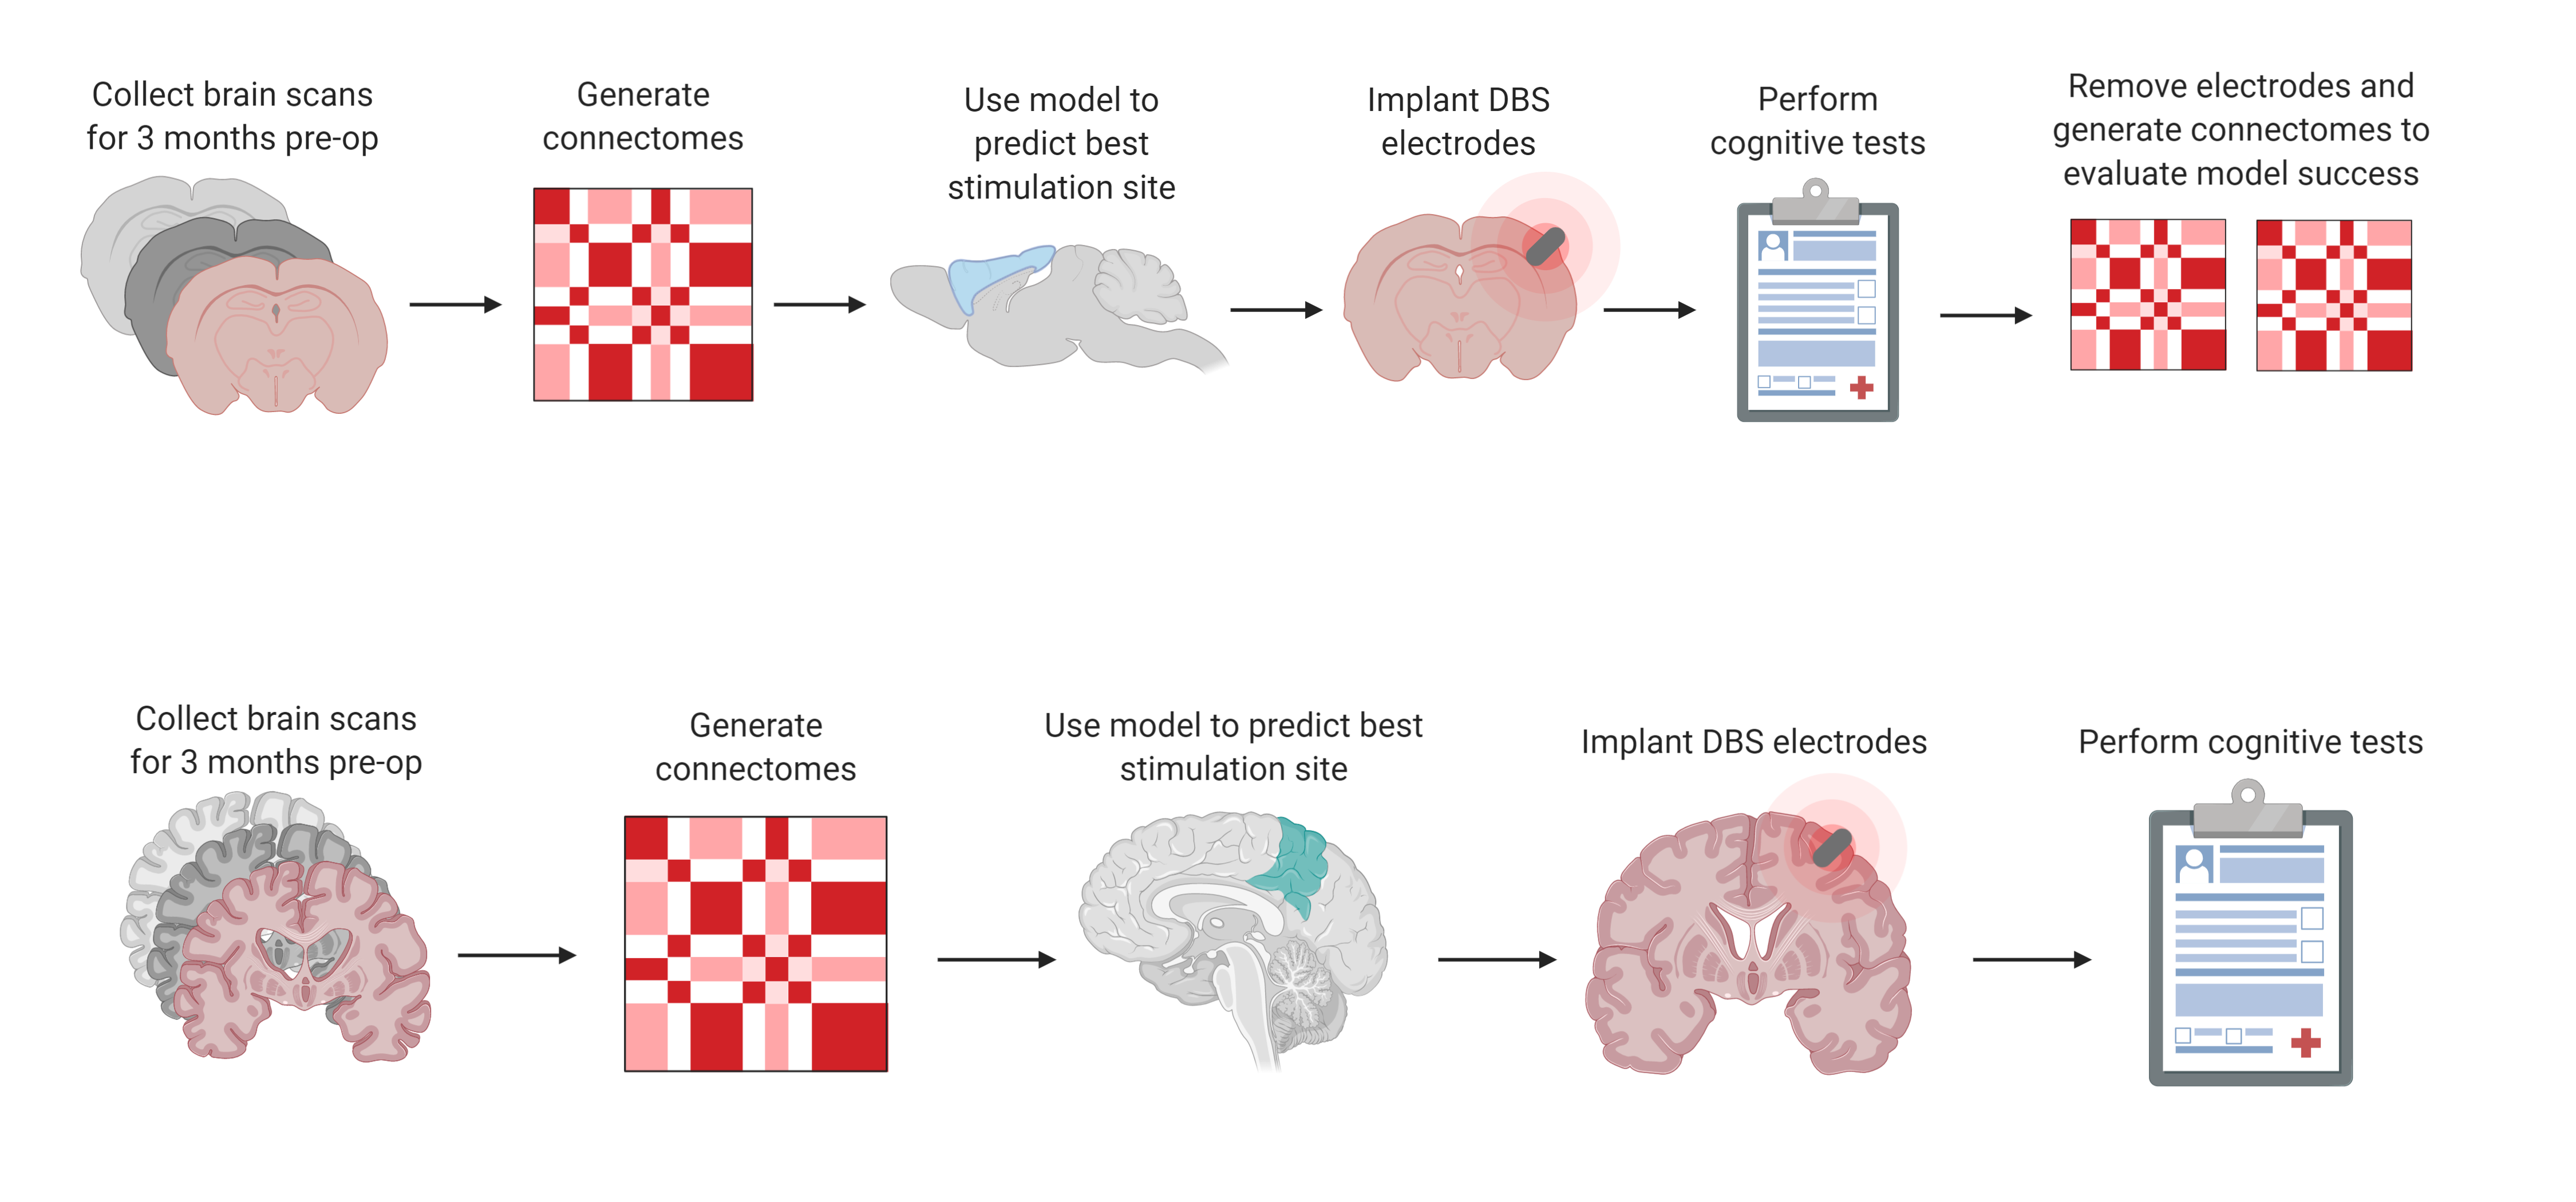
\includegraphics[width=120mm, scale=0.5]{Connectomics.png}
\caption{General overview of study methods}
\label{fig:method}
\end{figure}

\section{Data Collection}
For the purposes of this project, we wish to divide all experimentation into three segments - data collection, treatment, and testing. Our subject groups will consist of 100 mice and 100 humans. There will be four different age groups with 25 patients in each group for the human subjects:

Group 1: 35-50 years old

Group 2: 50-65 years old

Group 3: 65-75 years old

Group 4: 75+ years old

Twelve out of the subjects in each age group and mice cohort will be our control group. They will be mice and human subjects that have Alzheimer's but will not undergo DBS. This leaves 13 subjects in each group and cohort that will undergo DBS.

\subsection{fMRI and DTI Data Collection}
fMRI and diffusion tensor imaging (DTI) will be performed at different time points during a one-year progression of Alzheimer's disease in mice and human subjects (about 6-8 times during the year).

\subsection{Deep Brain Stimulation (DBS)}
The fMRI and DTI data will be used to generate brain connectomes for all patients. We wish to carry out this patient-directed treatment because the rate and progression of Alzheimer's disease differs greatly between patients. We hope to apply an algorithm to the connectomes that will provide us with information regarding the rate at which each affected brain area is changing, and which new areas are most likely to be affected. The purpose of this is to determine which brain regions the electrodes should be placed. Both the mice and human patients will under deep brain stimulation over the course of a year and a half. The idea is that DBS will yield positive results if electrodes are placed in the regions that are changing at a faster rate. In the human patients, nothing will be done immediately with the regions that are predicted to become affected during the progression of Alzheimer's. However, they will be used to check the accuracy of our prediction over time. Because of the presesnce of electrodes, our patients will not have fMRI and DTI scans performed after DBS treatment; only the mice that will undergo scanning after treatment.

\subsection{Behavior Tests}
To examine the effectiveness of the DBS on the human patients, we will perform various behavior tests such as memory and attention tests. We should not be surprised if deep brain stimulation does not yield positive results in the older age group because a decline in cognitive functioning is common in Parkinson's patients over 70 years of age undergoing DBS.
Because the mice will get fMRI and DTI scanning after DBS treatment, behavior tests are not compulsory. The post-DBS scans for the mice will serve as an effective method to see if Alzheimer's progression has decreased, increased or stayed the same.

\section{Data Processing and Information Extraction}
An automated pipeline will be used to create connectome data before and after Deep Brain Stimulation. \cite{Pipeline} Graph analysis will be conducted between the images to detect any noticeable changes. Statistical analysis will determine whether these changes are indicative of any improvements in the subject's condition. The level of computation needed to process 1mm voxel size image data sets can be done locally rather quickly or by sending jobs to a super computer.

\begin{figure}[h!]
\centering
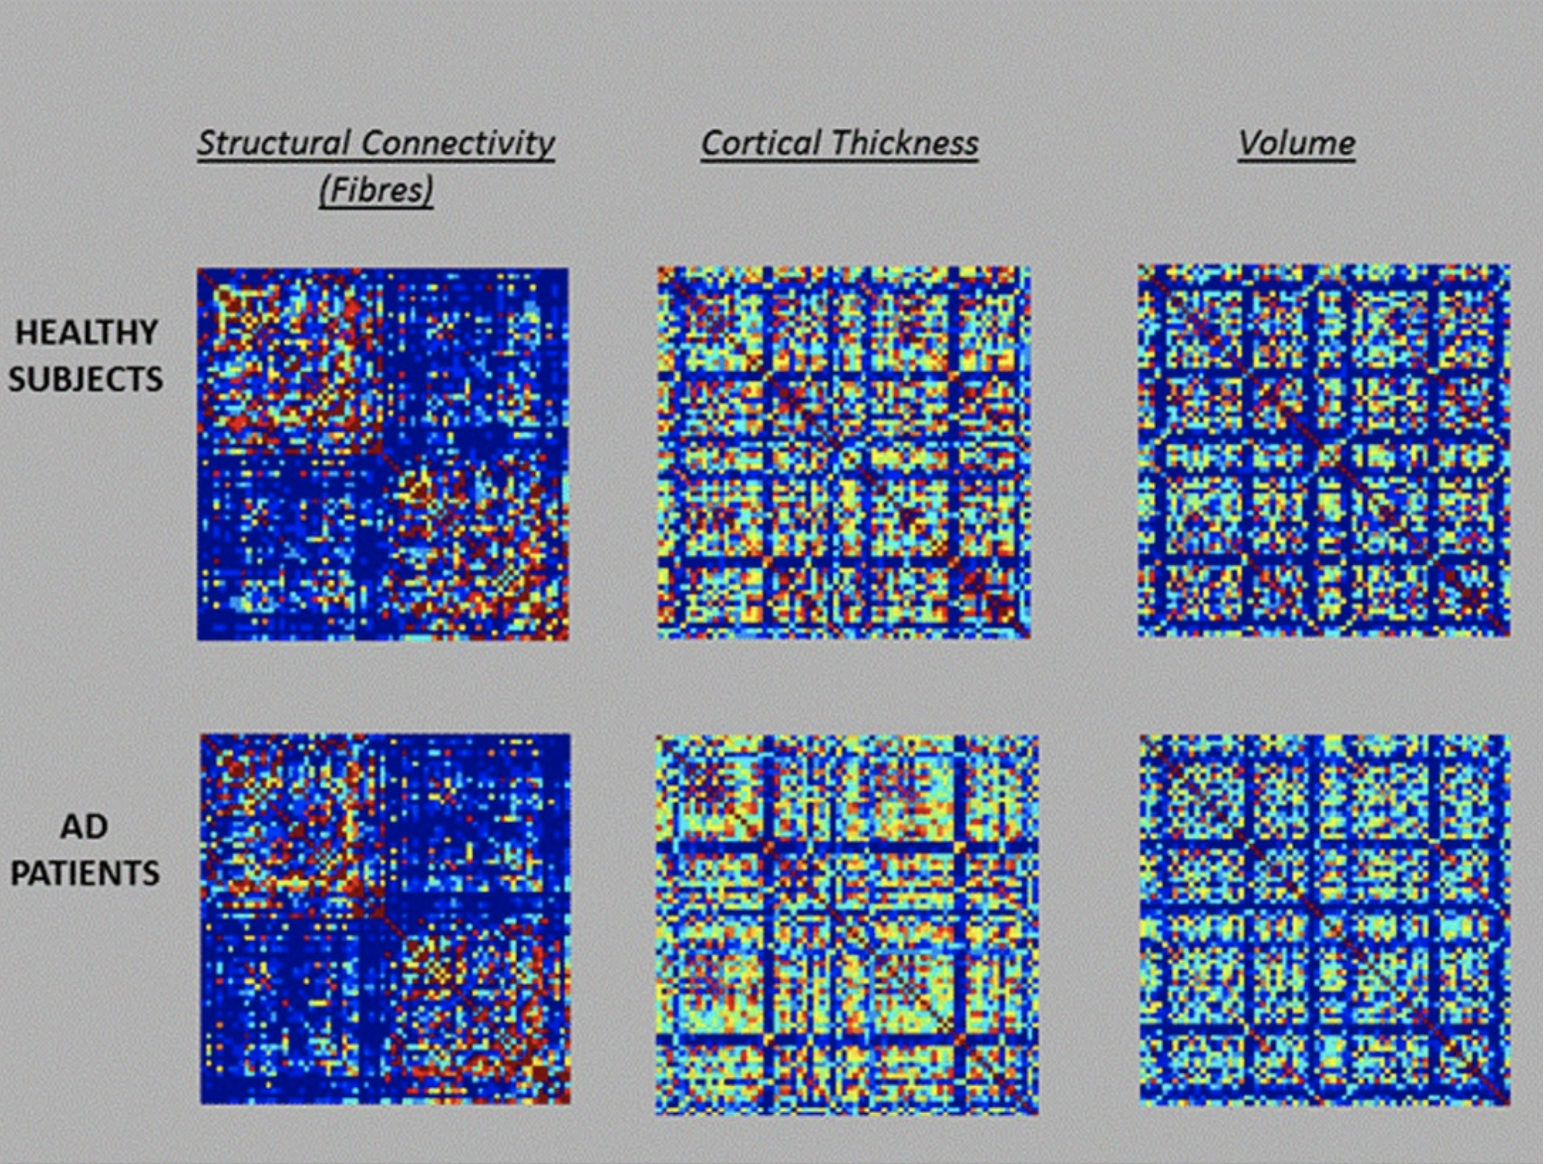
\includegraphics[width=75mm, scale=1]{matrix}
\caption{Here is a similar process conducted without DBS. \cite{Pipeline}}
\label{fig:method}
\end{figure}
\section{Data Storage}
    Data upload and storage will be done through Amazon Web Services. The prices are up to date as of 1/23/20.
\subsection{Short-Term Quick Access}
    The cost for uploading data online for quick public access is $1150$ per month and $13800$ per year for the first 50tb of data. We do not expect to produce data sets larger than this considering the low resolution of MRI images. \cite{AWS}
\subsection{Long-Term Slow Access}
    The cost for uploading data online for delayed private access is $200$ per month and $24000$ per 10 years for 50tb. \cite{AWS}

\section{Estimated Cost}



\begin{thebibliography}{9}

\bibitem{Alzheimer's Facts} 
National Institute on Aging. 
\textit{Alzheimer's Disease Fact Sheet}. 
National Institute on Aging, National Institutes of Health, Bethesda, Maryland, 2019.
\\\texttt{https://www.nia.nih.gov/health/alzheimers-disease-fact-sheet}

\bibitem{AWS}
Amazon Web Services.
\textit{Amazon S3 pricing}
\\\texttt{https://aws.amazon.com/s3/pricing/?nc=sn\&loc=4}

\bibitem{DBS uses} 
Mayo Clinic Staff. 
\textit{Deep Brain Stimulation}. 
Mayo Clinic, 2020.
\\\texttt{https://www.mayoclinic.org/tests-procedures/deep-brain-stimulation/about/pac-20384562}

\bibitem{DBS PD} 
Little, S., Beudel, M., Zrinzo, L., Foltynie, T., Limousin, P., Hariz, M., Neal, S., Cheeran, B., Cagnan, H., Gratwicke, J., Aziz, T.Z., Pogosyan, A., Brown, P. 
\textit{Bilateral adaptive deep brain stimulation is effectivein Parkinson’s disease}. 
J Neurol Neurosurg Psychiatry, 2016; 87:717–721.

\bibitem{DBS AD} 
Lozano, A. M., Fosdick, L., Chakravarty, M. M., Leoutsakos, J. M., Munro, C., Oh, E., … Smith, G. S. 
\textit{A Phase II Study of Fornix Deep Brain Stimulation in Mild Alzheimer’s Disease}. 
Journal of Alzheimer's disease, 54(2), 777–787. 

\bibitem{DBS for Parkinson's}
Jennifer A. Foley, Tom Foltynie, Patricia Limousin, Lisa Cipolotti
\textit{Standardized Neuropsychological Assessment for the Selection of Patients Undergoing DBS for Parkinson's Disease}.
Parkinson's Disease, Hindawi, 3 June 2018.
\\\texttt{https://www.ncbi.nlm.nih.gov/pmc/articles/PMC6009029/}

\bibitem{DBS and Parkinson's}
Andreas Horn, Martin Reich, Johannes Vorwerk, Ningfei Li, Gregor Wenzel, Qianqian Fang, Tanja Schmitz-Hübsch, Robert Nickl, Andreas Kupsch, Jens Volkmann, Andrea A. Kühn, Michael D. Fox.
\textit{Connectivity Predicts Deep Brain Stimulation Outcome in Parkinson Disease}
Annals of Neurology, U.S. National Library of Medicine, July 2017.
\\\texttt{https://www.ncbi.nlm.nih.gov/pmc/articles/PMC5880678/}

\bibitem{Pipeline}
Andre Santos Ribeiro, Luis Miguel Lacerda, Nuno Andre da Silva, Hugo Alexandre Ferreira.
\textit{Multimodel imaging brainy connectivity analysis (MIBCA) toolbox: preliminary application to Alzheimer's disease}
EJNMMI physics vol. 1, 2014.
\\\texttt{https://www.ncbi.nlm.nih.gov/pmc/articles/PMC4545458/}

\end{thebibliography}

\end{document}
